\documentclass[conference]{IEEEtran}
\usepackage{graphicx}
\usepackage{booktabs}
\usepackage{amsmath}
\usepackage{url}
\usepackage{cite}
\usepackage[hidelinks]{hyperref}
\usepackage{xcolor}
\usepackage{adjustbox}

% generated by paper/build.py from summary.json (2026-11-01T18:21:06)
\newcommand{\ComponentDetectionFOPipeline}{53.1}
\newcommand{\ComponentDetectionFOBaseline}{25.6}
\newcommand{\ComponentDetectionFOCv}{42.9}
\newcommand{\ComponentDetectionFOVision}{33.5}
\newcommand{\ComponentDetectionFODomPipeline}{42.9}
\newcommand{\ComponentDetectionFODomBaseline}{25.6}
\newcommand{\WhisperWerPipeline}{4.0}
\newcommand{\WhisperWerBaseline}{--}
\newcommand{\WhisperWerMeanPerCommand}{4.1}
\newcommand{\WhisperWerExactTranscripts}{85.0}
\newcommand{\VoiceCommandAccuracyPipeline}{91.2}
\newcommand{\VoiceCommandAccuracyBaseline}{--}
\newcommand{\VoiceCommandAccuracyFromText}{93.8}
\newcommand{\VisualSimilarityLayoutIouPipeline}{39.9}
\newcommand{\VisualSimilarityLayoutIouBaseline}{28.3}
\newcommand{\VisualSimilarityEdgeSsimPipeline}{52.2}
\newcommand{\VisualSimilarityEdgeSsimBaseline}{50.9}
\newcommand{\FunctionalCorrectnessPipeline}{94.8}
\newcommand{\FunctionalCorrectnessBaseline}{86.2}
\newcommand{\RequirementSatisfactionPipeline}{87.5}
\newcommand{\RequirementSatisfactionBaseline}{86.0}
\newcommand{\RefinementSuccessRatePipeline}{95.0}
\newcommand{\RefinementSuccessRateBaseline}{90.0}
\newcommand{\RefinementSuccessRatePipelineFromWhisper}{93.8}
\newcommand{\PreservationRatePipeline}{99.8}
\newcommand{\PreservationRateBaseline}{98.2}
\newcommand{\ValidationPassRateBeforeRepairPipeline}{100.0}
\newcommand{\ValidationPassRateBeforeRepairBaseline}{--}
\newcommand{\ValidationPassRateAfterRepairPipeline}{100.0}
\newcommand{\ValidationPassRateAfterRepairBaseline}{--}
\newcommand{\FaultDetectionRatePipeline}{96.8}
\newcommand{\FaultDetectionRateBaseline}{--}
\newcommand{\FaultRepairRatePipeline}{73.5}
\newcommand{\FaultRepairRateBaseline}{--}
\newcommand{\GenerationTimeMsPipeline}{15.5}
\newcommand{\GenerationTimeMsBaseline}{24.0}
\newcommand{\GenerationTimeMsPipelineMedian}{10.7}
\newcommand{\GenerationTimeMsPipelinePNF}{18.3}
\newcommand{\GenerationTimeMsBaselineMedian}{17.0}
\newcommand{\GenerationTimeMsBaselinePNF}{65.2}
\newcommand{\GenerationTimeMsPipelineWithValidationMean}{16.4}
\newcommand{\ModificationTimeMsPipeline}{2.1}
\newcommand{\ModificationTimeMsBaseline}{15.4}
\newcommand{\ModificationTimeMsPipelineMedian}{2.1}
\newcommand{\ModificationTimeMsBaselineMedian}{13.9}
\newcommand{\CodeParseRatePipeline}{100.0}
\newcommand{\CodeParseRateBaseline}{100.0}
\newcommand{\CodeEslintMessagesPipeline}{0.05}
\newcommand{\CodeEslintMessagesBaseline}{0.03}
\newcommand{\CodeReuseRatioPipeline}{1.9}
\newcommand{\CodeReuseRatioBaseline}{1.0}
\newcommand{\CodeMaxFunctionLinesPipeline}{105.6}
\newcommand{\CodeMaxFunctionLinesBaseline}{206.1}
\newcommand{\CountSketches}{40}
\newcommand{\CountCommands}{80}
\newcommand{\CountCategories}{10}
\newcommand{\CountGtComponents}{490}
\newcommand{\ApiCalls}{480}

% generated by paper/build.py from summary.json (2026-11-01T01:35:57)
\newcommand{\DevComponentDetectionFOPipeline}{42.9}
\newcommand{\DevComponentDetectionFOBaseline}{25.6}
\newcommand{\DevComponentDetectionFOCv}{37.0}
\newcommand{\DevComponentDetectionFOVision}{8.8}
\newcommand{\DevComponentDetectionFODomPipeline}{16.5}
\newcommand{\DevComponentDetectionFODomBaseline}{25.6}
\newcommand{\DevWhisperWerPipeline}{4.0}
\newcommand{\DevWhisperWerBaseline}{--}
\newcommand{\DevWhisperWerMeanPerCommand}{4.1}
\newcommand{\DevWhisperWerExactTranscripts}{85.0}
\newcommand{\DevVoiceCommandAccuracyPipeline}{95.0}
\newcommand{\DevVoiceCommandAccuracyBaseline}{--}
\newcommand{\DevVoiceCommandAccuracyFromText}{96.2}
\newcommand{\DevVisualSimilarityLayoutIouPipeline}{20.5}
\newcommand{\DevVisualSimilarityLayoutIouBaseline}{28.3}
\newcommand{\DevVisualSimilarityEdgeSsimPipeline}{51.6}
\newcommand{\DevVisualSimilarityEdgeSsimBaseline}{50.9}
\newcommand{\DevFunctionalCorrectnessPipeline}{91.4}
\newcommand{\DevFunctionalCorrectnessBaseline}{86.2}
\newcommand{\DevRequirementSatisfactionPipeline}{86.0}
\newcommand{\DevRequirementSatisfactionBaseline}{86.0}
\newcommand{\DevRefinementSuccessRatePipeline}{81.2}
\newcommand{\DevRefinementSuccessRateBaseline}{90.0}
\newcommand{\DevRefinementSuccessRatePipelineFromWhisper}{83.8}
\newcommand{\DevPreservationRatePipeline}{97.7}
\newcommand{\DevPreservationRateBaseline}{98.2}
\newcommand{\DevValidationPassRateBeforeRepairPipeline}{42.5}
\newcommand{\DevValidationPassRateBeforeRepairBaseline}{--}
\newcommand{\DevValidationPassRateAfterRepairPipeline}{42.5}
\newcommand{\DevValidationPassRateAfterRepairBaseline}{--}
\newcommand{\DevFaultDetectionRatePipeline}{83.6}
\newcommand{\DevFaultDetectionRateBaseline}{--}
\newcommand{\DevFaultRepairRatePipeline}{60.7}
\newcommand{\DevFaultRepairRateBaseline}{--}
\newcommand{\DevGenerationTimeMsPipeline}{21.9}
\newcommand{\DevGenerationTimeMsBaseline}{24.0}
\newcommand{\DevGenerationTimeMsPipelineMedian}{16.0}
\newcommand{\DevGenerationTimeMsPipelinePNF}{57.5}
\newcommand{\DevGenerationTimeMsBaselineMedian}{17.0}
\newcommand{\DevGenerationTimeMsBaselinePNF}{65.2}
\newcommand{\DevGenerationTimeMsPipelineWithValidationMean}{23.3}
\newcommand{\DevModificationTimeMsPipeline}{2.7}
\newcommand{\DevModificationTimeMsBaseline}{15.4}
\newcommand{\DevModificationTimeMsPipelineMedian}{2.1}
\newcommand{\DevModificationTimeMsBaselineMedian}{13.9}
\newcommand{\DevCodeParseRatePipeline}{100.0}
\newcommand{\DevCodeParseRateBaseline}{100.0}
\newcommand{\DevCodeEslintMessagesPipeline}{0.07}
\newcommand{\DevCodeEslintMessagesBaseline}{0.03}
\newcommand{\DevCodeReuseRatioPipeline}{2.0}
\newcommand{\DevCodeReuseRatioBaseline}{1.0}
\newcommand{\DevCodeMaxFunctionLinesPipeline}{57.3}
\newcommand{\DevCodeMaxFunctionLinesBaseline}{206.1}
\newcommand{\DevCountSketches}{40}
\newcommand{\DevCountCommands}{80}
\newcommand{\DevCountCategories}{10}
\newcommand{\DevCountGtComponents}{490}
\newcommand{\DevApiCalls}{480}


\begin{document}

\title{NeuroGenUI: Multimodal Sketch-and-Voice Generation of Editable, Validated User Interfaces through a Structured UI Intent Representation}

\author{\IEEEauthorblockN{Author One, Author Two, Author Three}
\IEEEauthorblockA{Department of Computer Science and Engineering\\
Institution Name, City, Country\\
\{author1, author2, author3\}@institution.edu}}

\maketitle

\begin{abstract}
We present NeuroGenUI, a multimodal framework that generates editable React user interfaces from a hand-drawn sketch and spoken instructions, and refines them with further voice commands. Instead of a single image-to-code call, the system separates perception, interpretation, fusion, generation and validation around an explicit JSON UI Intent Representation: OpenCV proposals are labelled by a vision model, speech is transcribed by Whisper and converted into typed edit operations, a deterministic geometry-aware compiler emits React code, and a headless-browser validator drives a targeted repair loop. We evaluate every stage on \CountSketches{} labelled synthetic sketches and \CountCommands{} synthetic spoken commands, against a direct sketch-to-UI baseline using the same model and measurement code. On rendered UIs, the pipeline detects the sketched components with F1 \ComponentDetectionFODomPipeline{}\% versus \ComponentDetectionFODomBaseline{}\%, passes \FunctionalCorrectnessPipeline{}\% of specified interactions versus \FunctionalCorrectnessBaseline{}\%, and applies refinements in \ModificationTimeMsPipeline{}\,s versus \ModificationTimeMsBaseline{}\,s while preserving \PreservationRatePipeline{}\% of unaffected components; requirement satisfaction and refinement success are at parity with the baseline. Fault injection shows the validator detects \FaultDetectionRatePipeline{}\% of injected faults and the repair loop restores \FaultRepairRatePipeline{}\%. An initial evaluation exposed defects that were fixed on the same test set, so results are development-set figures on synthetic data. Code, dataset and evaluation scripts are provided.
\end{abstract}


\begin{IEEEkeywords}
sketch-to-code, multimodal interaction, speech interfaces, UI generation, large language models, program validation, automated repair
\end{IEEEkeywords}

\section{Introduction}
Designers usually start a user interface (UI) with a rough sketch on paper or a whiteboard. Turning that sketch into working front-end code is slow and repetitive, and the sketch itself only says \emph{where} things are: it does not say what a field validates, where a button navigates, or which colour a primary action should have. People state that kind of intent naturally in speech (``when the login button is clicked, show an error if the fields are empty''), not in drawings.

Recent vision--language models can turn a screenshot or sketch into code in a single call~\cite{si2024design2code}. That single-call approach has three practical weaknesses for interactive design. First, its intermediate understanding is hidden inside the model, so detection, interpretation and generation cannot be measured or corrected separately. Second, every modification regenerates the whole program, which is slow and can silently change parts the user did not ask to change. Third, nothing checks that the produced UI actually renders, contains what was sketched, or behaves as requested.

This paper presents \textbf{NeuroGenUI}, a multimodal framework that combines a hand-drawn sketch with spoken instructions through an explicit, structured \emph{UI Intent Representation} (IR). Each stage is separate and measurable: OpenCV proposes candidate components and a vision model labels them (hybrid detection); Whisper~\cite{radford2023whisper} transcribes speech; a language model interprets the transcript into typed edit operations without ever writing code; a deterministic fusion step merges sketch geometry with spoken semantics into the IR; a deterministic compiler emits an editable React project; a headless-browser validator checks visual and functional properties; and a targeted repair loop fixes the specific component that failed. Spoken refinements are applied as operations on the existing IR, so unaffected components are preserved by construction.

The contributions of this work are:
\begin{itemize}
\item A staged sketch\,+\,voice $\rightarrow$ IR $\rightarrow$ React architecture in which no stage is a single image-to-code call and every stage is timed and evaluated in isolation.
\item A JSON UI Intent Representation that carries type, content, geometry, style, hierarchy, relations and event/action semantics, together with a typed operation language for voice-guided refinement.
\item A validation and targeted repair loop that runs the generated code in a real browser and maps failing checks back to IR components.
\item An open evaluation protocol with \CountSketches{} labelled sketches across \CountCategories{} screen categories and \CountCommands{} spoken commands across eight edit categories, and a like-for-like comparison against a direct sketch$\rightarrow$AI$\rightarrow$UI baseline using the same model, the same test cases and the same measurement code.
\end{itemize}
We do not train a new foundation model; the contribution is the system architecture and its measurement. All numbers in this paper are produced by the released evaluation scripts.

\section{Related Work}
\textbf{Sketch-based UI design.} SILK~\cite{landay1995silk} showed early that electronic sketching supports the exploratory stage of UI design and that sketched widgets can be recognised and made interactive. Later systems learned the mapping from images to code: pix2code~\cite{beltramelli2018pix2code} generated a domain-specific language from screenshots with a CNN--LSTM, ReDraw~\cite{moran2020redraw} classified detected mobile components and assembled them into app code, and several Sketch2Code systems~\cite{robinson2019sketch2code,jain2019sketch2code} produced web pages from paper mockups with object detection and heuristics. Large UI corpora such as Rico~\cite{deka2017rico} enabled data-driven design tools. These systems are vision-only: behaviour, navigation and styling intent cannot be expressed in the sketch and are therefore absent from the output.

\textbf{LLM-based front-end generation.} General multimodal models~\cite{openai2023gpt4} can produce HTML/React from an image in one call, and Design2Code~\cite{si2024design2code} benchmarks this ability on real web pages. Our baseline follows this direct approach. Our work differs in that the model is used only for perception (labelling proposals, reading handwriting) and interpretation (speech to typed operations), while code generation, refinement and repair are deterministic operations on an explicit representation.

\textbf{Multimodal and voice interaction.} Combining speech with a spatial channel goes back to ``Put-That-There''~\cite{bolt1980put}. Modern speech recognisers such as Whisper~\cite{radford2023whisper} make spoken commands practical. NeuroGenUI uses speech for the information a sketch cannot carry: semantics, behaviour and edits to an existing design.

\textbf{Iterative refinement and repair.} Self-refinement methods let language models critique and revise their own output~\cite{madaan2023selfrefine}. Our repair loop is instead grounded in executable checks: the generated UI is rendered in a headless browser, failures are attributed to specific IR components, and only those components are changed before revalidation.

\section{System Architecture}
\begin{figure*}[t]
\centering
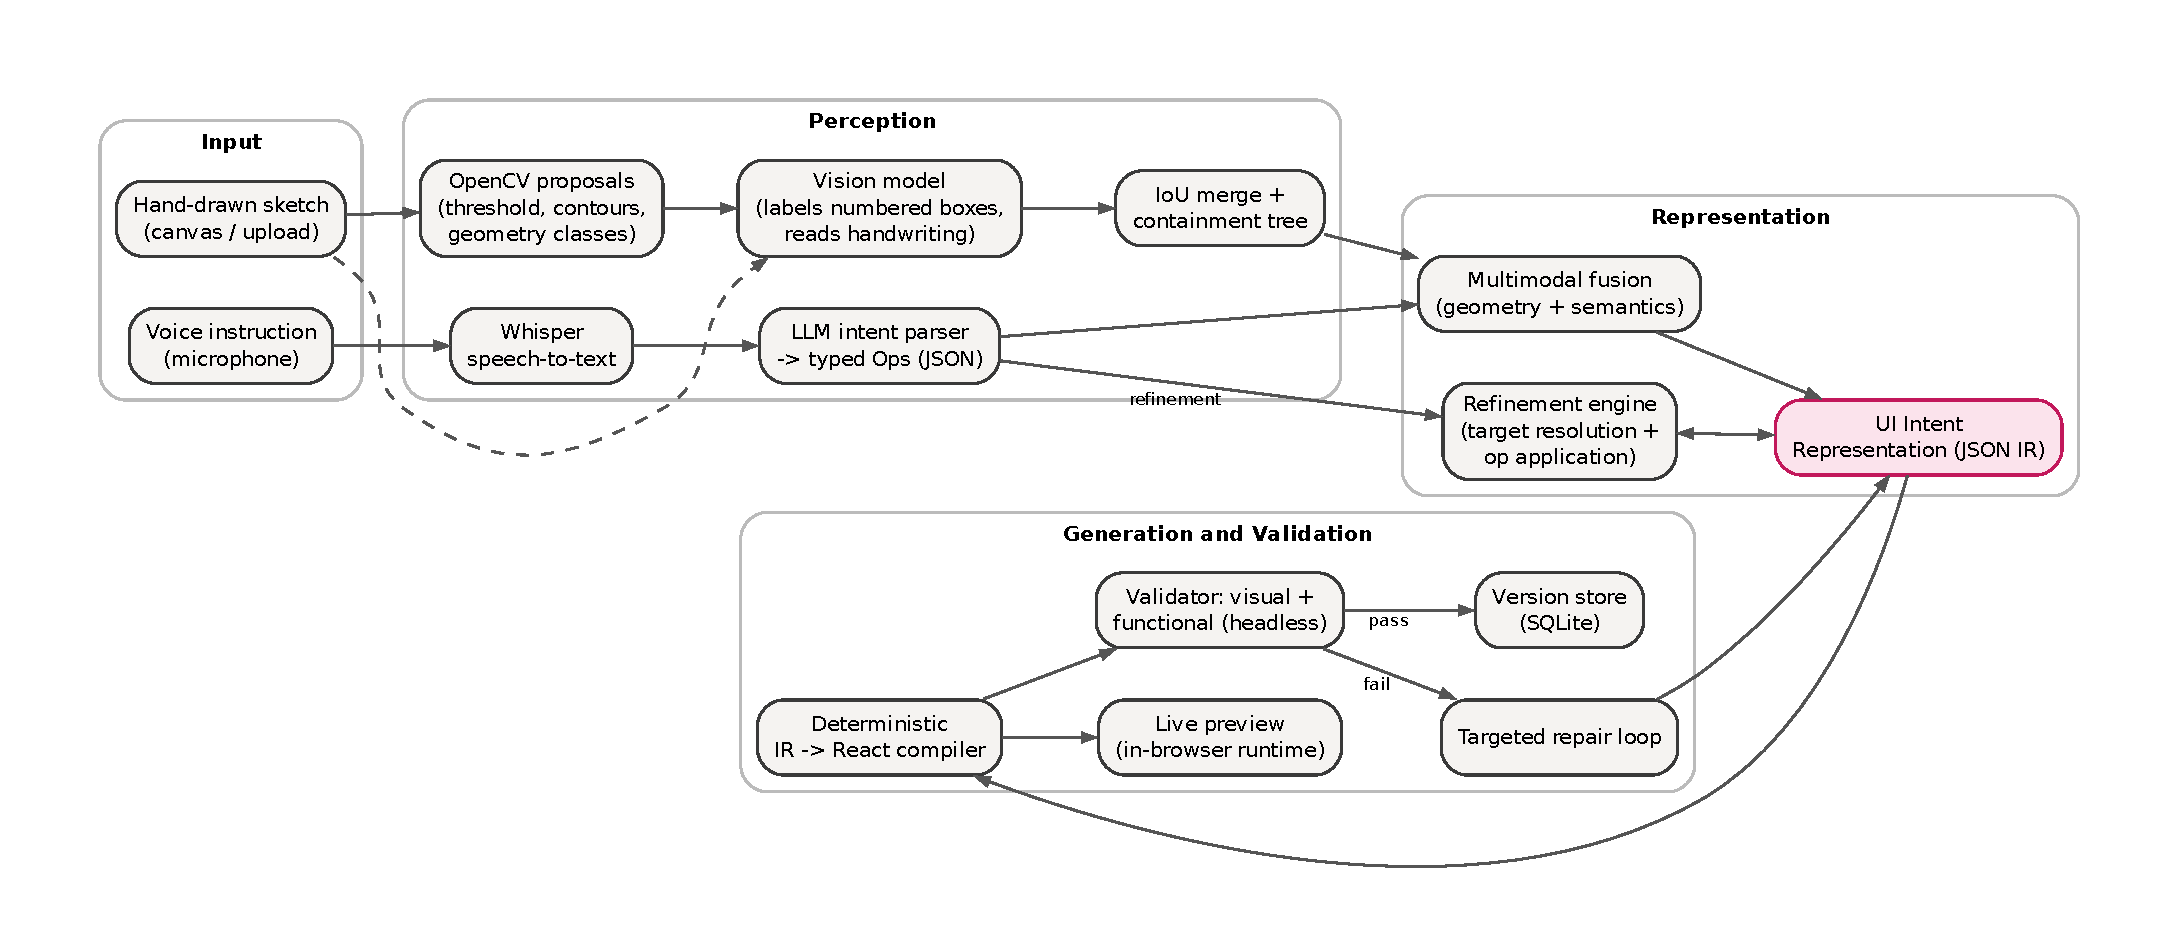
\includegraphics[width=0.92\textwidth]{figures/architecture.pdf}
\caption{NeuroGenUI architecture. Perception (OpenCV proposals, vision labelling, Whisper, LLM intent parsing) feeds a deterministic fusion step that produces the JSON UI Intent Representation (IR). The IR is compiled to React, rendered live, validated in a headless browser and repaired; voice refinements edit the IR rather than regenerating code.}
\label{fig:arch}
\end{figure*}

Fig.~\ref{fig:arch} shows the architecture and Fig.~\ref{fig:flow} the interaction flow. The stages are independent modules with fixed interfaces, each timed separately by the orchestrator (\texttt{upload}, \texttt{analyze\_sketch}, \texttt{transcribe}, \texttt{interpret}, \texttt{fuse}, \texttt{codegen}, \texttt{validate}, \texttt{repair}, \texttt{save}).

\subsection{Sketch Understanding}
\label{sec:sketch}
\textit{OpenCV proposals.} The sketch is converted to grayscale, binarised with adaptive thresholding and closed morphologically so that wobbly, non-closed hand-drawn strokes join into contours. Contours are extracted with their hierarchy~\cite{suzuki1985topological,bradski2000opencv}, approximated by polygons and classified by geometry: small squares become checkbox candidates, small circles radio candidates, wide short rectangles input or button candidates, rectangles crossed by diagonals image placeholders, long thin strokes dividers, and clusters of small strokes handwritten text.

\textit{Vision labelling.} The candidate boxes are drawn with numeric tags onto a copy of the sketch, and a vision model (GPT-4.1-mini) receives this annotated image. Under a JSON schema it assigns each numbered box a component type from the IR vocabulary, transcribes its handwritten text, and adds components the proposals missed. The model therefore classifies and reads but does not localise from scratch.

\textit{Merge.} Vision labels are attached to proposals, added components are merged by IoU, and a containment tree assigns parents. Three modes are available for ablation: \texttt{cv} (geometry only), \texttt{vision} (the model alone, boxes included) and \texttt{hybrid} (the proposed combination).

\subsection{Speech and Intent Understanding}
Speech recorded in the browser is transcribed with Whisper (\texttt{whisper-1}). A language model (GPT-4.1-mini, temperature 0, JSON-schema output) converts the transcript into a list of typed \emph{operations}: \texttt{create}, \texttt{add}, \texttt{remove}, \texttt{modify}, \texttt{move}, \texttt{resize}, \texttt{style}, \texttt{interaction} and \texttt{navigation}. When an IR exists, the model sees a compact outline of it (id, type, label, parent) so it can name targets directly. An operation carries a target reference, an optional new component, a relative position (\emph{below}, \emph{above}, \emph{left\_of}, \emph{right\_of}, \emph{inside}), property and style changes, or an event with actions. The model never writes code.

\subsection{UI Intent Representation}
The IR is a JSON document with pages, each holding a component tree. Every node has a stable id, a type (page, container, card, form, header, navbar, nav item, heading, text, link, button, input, textarea, checkbox, radio, select, image, list, divider, icon), a label, type-specific properties (input type, placeholder, required flag, options), style (variant, colour, size, width, alignment), container layout, a normalised bounding box from the sketch, relations to other nodes, and events. Events bind a trigger (click, submit, change) to an ordered list of actions: \texttt{validate\_required}, \texttt{validate\_format}, \texttt{show\_message}, \texttt{navigate}, \texttt{toggle\_visibility} and \texttt{set\_text}.

\subsection{Multimodal Fusion}
Fusion is deterministic. The sketch decides \emph{where} things are: components are grouped into rows by vertical overlap, containment (by box centre) gives parents, side-by-side columns are detected, and drawn plain containers become cards or forms. The voice description decides \emph{what} they are: input types, required flags, events and the page title. Matching runs in two passes. First, spoken and sketched components with near-identical labels are paired globally, and text-like types count as compatible. Second, each remaining spoken component is matched by type compatibility and reading order between its already-anchored neighbours. A spoken component whose label matches a drawn one is never inserted a second time. When drawn and spoken text disagree, the drawn text is kept and the voice contributes properties and behaviour. Unmatched spoken components are inserted next to their spoken neighbours, and unmatched sketched components are kept. Before fusion, the analysis is cleaned: fragments of one handwritten word are merged, duplicate detections of the same text are removed, and labels that contradict the drawn shape fall back to the geometric class.

\subsection{Code Generation and Live Preview}
A deterministic compiler translates the IR into a React project: one reusable component per IR type (\texttt{Button}, \texttt{Field}, \texttt{Heading}, \texttt{Card}, \dots), one component per page, a state-based router, and event handlers that call a small action runtime. The compiler is \emph{geometry-aware}: the page frame (phone or desktop) follows the sketch's aspect ratio, and each node's normalised sketch box becomes widths and offsets proportional to its parent, vertical spacing proportional to the drawing, and drawn heights for images, buttons and boxes. All of this is expressed with flex rows and columns that wrap on narrow screens rather than absolute positioning, so the code stays responsive and readable. Explicit user styles always override geometry. The output is a runnable Vite project that the user can export and edit, plus a single-script form that the browser runtime transpiles with Babel and renders live in an iframe. Because the compiler is deterministic, the same IR always yields the same code, and a local IR edit yields a local code change.

\subsection{Voice-Guided Refinement}
A spoken refinement is transcribed and interpreted into operations against the current IR. Targets are resolved by the id the model supplied when it is valid, otherwise by a deterministic resolver that scores type keywords, fuzzy label similarity, ordinals (``the second button'') and position words. Application is pure: the IR is deep-copied, only targeted nodes change, untouched nodes stay byte-identical, and every operation reports success or a reason for failure. The changed IR is recompiled and the preview refreshes. Every result is stored as a new version with its transcript, operations, IR, code, validation report and stage timings, so iterative refinement can be inspected and restored.

\subsection{Validation and Targeted Repair}
\begin{figure}[t]
\centering
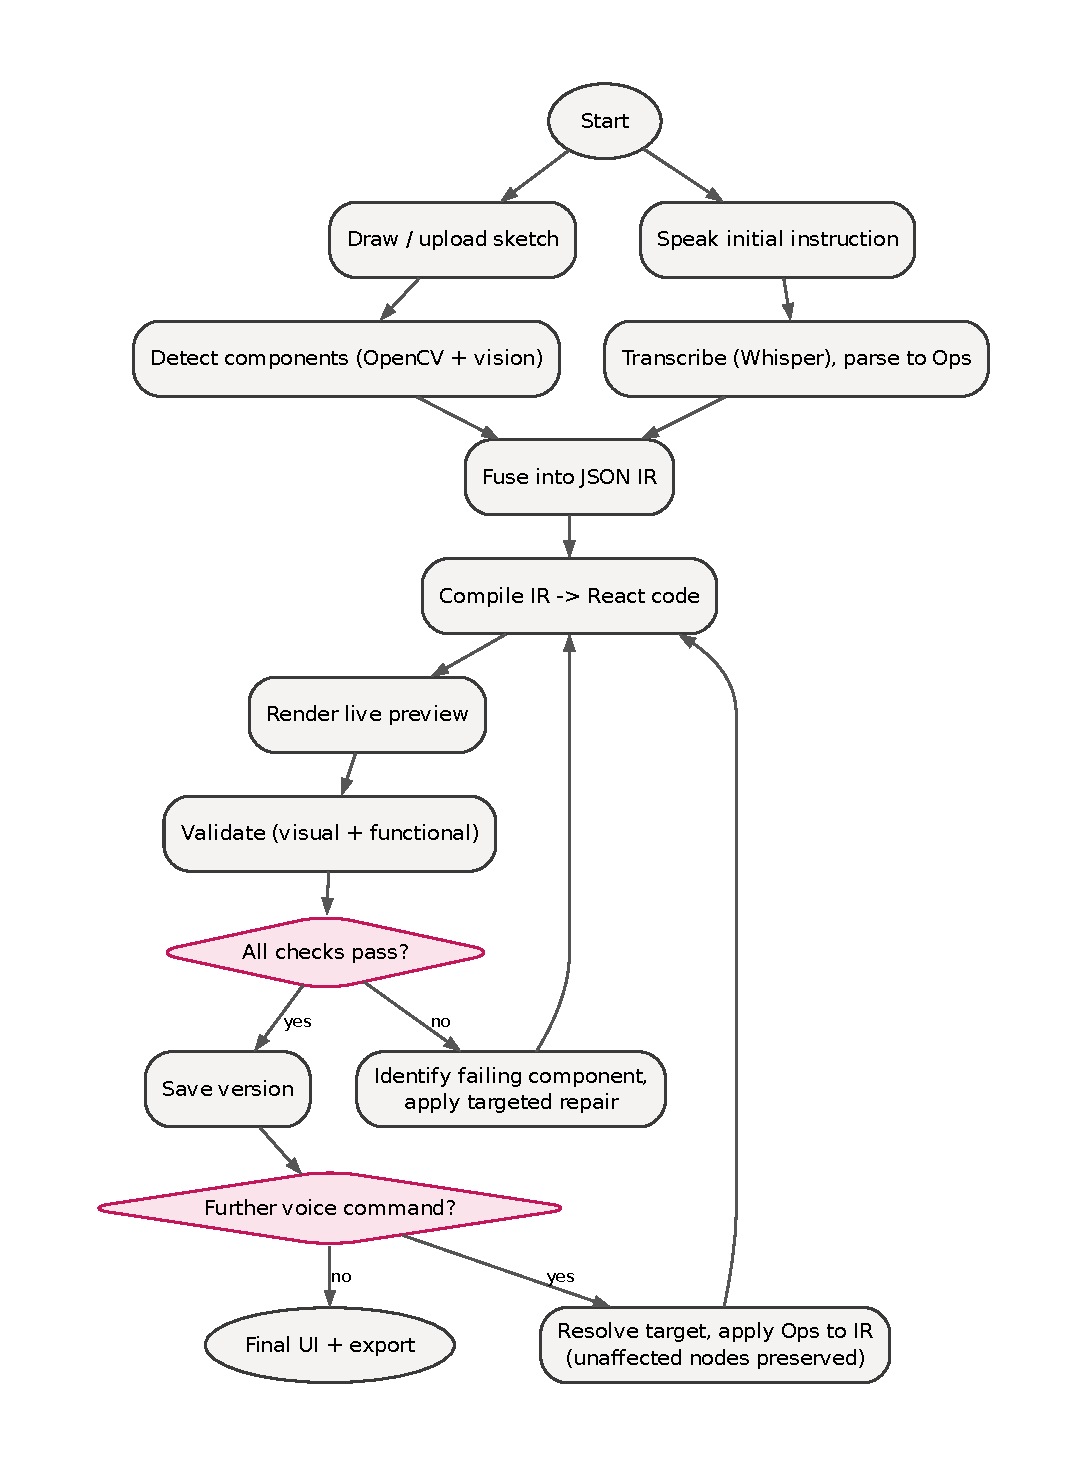
\includegraphics[width=0.78\columnwidth]{figures/flowchart.pdf}
\caption{Interaction flow with validation, targeted repair and iterative voice refinement.}
\label{fig:flow}
\end{figure}
The validator loads the generated code into the same runtime page the user sees, inside a headless browser (Playwright, Chromium or Edge). \textit{Visual checks} verify that every IR node is rendered and visible, that sibling order matches the IR and the sketch, that sketched components are covered, and the overlap between rendered boxes and sketch boxes. \textit{Functional checks} capture runtime and console errors, click every button, type into every input, and simulate every event to assert its effect (an error message for empty required fields, the target page after navigation, a visibility change after a toggle).

The repair loop maps each failing check to the responsible IR node and applies a targeted fix: a missing sketched component is re-inserted from the analysis, out-of-order siblings are reordered, a hidden or zero-size node has its style reset, a node missing from the DOM or a runtime error triggers recompilation in a safe mode, and a failing interaction has its handler rebuilt. The UI is then revalidated, up to three iterations. Repairs never undo an explicit user edit: removed and moved components are recorded in the IR metadata and excluded from coverage and order repairs.

\section{Experimental Setup}
\subsection{Dataset}
\textbf{Sketches.} We built \CountSketches{} UI sketches, four for each of \CountCategories{} screen categories: login, registration, dashboard, profile, e-commerce, banking, booking, contact, settings and landing page. Each screen is specified as a component tree with varied layouts (navigation bars, multi-column rows, cards, image placeholders, radio and checkbox groups, selects, multiple buttons). It is rendered in a hand-drawn style with jittered, overshooting multi-segment strokes, slightly rotated and non-closed rectangles, varying pen width, three handwriting fonts and paper noise. Ground truth (type, label, normalised box and parent for \CountGtComponents{} components) comes from the specification. Each sketch also has a natural spoken description used in the generation step, plus the interactions and requirements that description implies. The sketches are \emph{synthetic}; Section~\ref{sec:limits} discusses what this implies.

\textbf{Voice commands.} We wrote \CountCommands{} commands, ten for each of add, remove, modify, move, resize, style, interaction and navigation. They include all seven example commands of the project specification (e.g., ``Make the login button blue'', ``Add a forgot password link below the login button''). Each command is tied to a sketch, labelled with its expected operation, target and parameters, and has a machine-checkable post-condition evaluated on the rendered UI. Each command was synthesised to speech with a text-to-speech model, rotating six voices, so that Whisper transcribes real audio.

\subsection{Baseline}
The baseline is the direct \emph{sketch$\rightarrow$AI$\rightarrow$UI} approach: one call to the same vision model (GPT-4.1-mini) receives the sketch and the spoken instruction and returns a complete React program. Modification sends the previous program and the command, and receives a regenerated program. The baseline prompt is a competent, fair prompt, and its output follows the same runtime contract, so the same renderer measures both systems.

\subsection{Metrics}
All metrics are computed by the same code for both systems. Measurement never uses the pipeline's internal \texttt{data-ngid} attributes; components are recovered from the rendered DOM by tags, ARIA roles, input types and visual cues.
\begin{itemize}
\item \textit{Component detection}: Hungarian matching~\cite{kuhn1955hungarian} of predicted to ground-truth boxes (IoU $\geq 0.3$). A match counts as a true positive when the types agree. Precision, recall and F1 are micro-averaged. It is measured on the analysis output (\texttt{cv}/\texttt{vision}/\texttt{hybrid}) and on the rendered DOM of each system.
\item \textit{Voice command accuracy}: Whisper word error rate (WER), plus the share of commands whose operation type, target and parameters are all interpreted correctly, from both the reference text and the Whisper transcript.
\item \textit{Visual similarity}: mean layout IoU between ground-truth components and their assigned rendered elements, and SSIM~\cite{wang2004ssim} between dilated Canny~\cite{canny1986edge} edge maps of the sketch and the screenshot.
\item \textit{Functional correctness}: the share of specified interactions that work when simulated in the browser. \textit{Requirement satisfaction}: the share of instruction-derived requirements (named components, input types, behaviours) that are met.
\item \textit{Refinement success}: the share of commands whose post-condition holds on the refined UI. \textit{Preservation}: the share of non-target components unchanged in type, text, colour, size and font.
\item \textit{Validation pass rate} before and after repair, and a \textit{fault-injection} study: deleted, hidden, zero-size and reordered nodes, broken events and injected runtime errors, scored by whether the validator detects each fault and whether repair removes it.
\item \textit{Generation time} per stage and end to end, and \textit{code quality}: parse success, lines of code, components, reuse ratio (component usages per definition), longest function and ESLint messages.
\end{itemize}

\subsection{Implementation}
The backend is Python (FastAPI, OpenCV, Playwright, SQLite for projects and versions), and the studio front end is React. The models are GPT-4.1-mini for vision and intent and \texttt{whisper-1} for speech, through the OpenAI API. The evaluation reran every stage in-process with cached raw model outputs, so metrics can be recomputed without further API calls. The full run made \ApiCalls{} model calls.

\section{Results}
All results come from one full run over the \CountSketches{} sketches and \CountCommands{} commands (\ApiCalls{} cached model calls). Both systems use the same model, test cases and measurement code. Table~\ref{tab:headline} summarises every metric; the subsections discuss them. Differences on this test set are single-run, and several are small enough (a few commands out of 80) that we describe them as parity rather than wins.

\begin{table}[t]
\centering
\scriptsize
\caption{Headline results on the same 40 sketches and 80 commands (proposed vs.\ one-call baseline)}
\label{tab:headline}
\setlength{\tabcolsep}{3pt}
\begin{adjustbox}{max width=\columnwidth}
\begin{tabular}{lrrl}
\toprule
\textbf{Metric} & \textbf{Proposed} & \textbf{Baseline} & \textbf{Unit} \\
\midrule
Component detection F1 (analysis vs.\ baseline DOM) & 53.1 & 25.6 & \% \\
Component detection F1 (both on rendered DOM) & 42.9 & 25.6 & \% \\
Whisper word error rate & 4.0 & -- & \% \\
Voice command accuracy (from Whisper) & 91.2 & -- & \% \\
Visual similarity: layout IoU $\times$100 & 39.9 & 28.3 & IoU$\times$100 \\
Visual similarity: edge SSIM $\times$100 & 52.2 & 50.9 & SSIM$\times$100 \\
Functional correctness & 94.8 & 86.2 & \% \\
Requirement satisfaction & 87.5 & 86.0 & \% \\
Refinement success rate & 95.0 & 90.0 & \% \\
Preservation of unaffected components & 99.8 & 98.2 & \% \\
Validation pass rate before repair & 100.0 & -- & \% \\
Validation pass rate after repair & 100.0 & -- & \% \\
Injected faults detected & 96.8 & -- & \% \\
Injected faults repaired & 73.5 & -- & \% \\
Generation time, mean (s) & 15.5 & 24.0 & s \\
Modification time, mean (s) & 2.1 & 15.4 & s \\
Generated code parses & 100.0 & 100.0 & \% \\
ESLint messages per UI & 0.05 & 0.03 & count/UI \\
Component reuse ratio & 1.9 & 1.0 & usages/definition \\
Longest function (lines) & 105.6 & 206.1 & lines \\
\bottomrule
\end{tabular}
\end{adjustbox}
\end{table}


\subsection{Component Detection}
Table~\ref{tab:detection} separates the sketch-analysis stage from what is actually rendered. At the analysis stage, the hybrid detector reaches F1 \ComponentDetectionFOPipeline{}\% against \textbf{42.9\%} for OpenCV alone and \textbf{33.5\%} for the vision model alone, so neither component is sufficient. OpenCV localises well (mean IoU of matched boxes 0.72) but cannot read text or reliably tell types apart (type accuracy 52.9\%); the vision model labels well (87.7\% label accuracy) but localises loosely (mean IoU 0.52). Hybrid keeps OpenCV's boxes and the vision model's labels (95.3\% label accuracy).

The like-for-like comparison with the baseline is on the rendered DOM, because that is the only place the baseline's components exist. There the proposed pipeline scores F1 \ComponentDetectionFODomPipeline{}\% against \ComponentDetectionFODomBaseline{}\% for the baseline. A ground-truth oracle IR compiled by the same compiler scores 77.5\%, which bounds what the compiler achieves with perfect input and suggests that most of the remaining gap comes from upstream detection errors rather than code generation.

\begin{table*}[t]
\centering
\scriptsize
\caption{Component detection (micro-averaged; Hungarian matching, IoU $\geq$ 0.3, correct type)}
\label{tab:detection}
\setlength{\tabcolsep}{3.5pt}
\begin{adjustbox}{max width=\textwidth}
\begin{tabular}{lrrrrr}
\toprule
\textbf{Detector / output} & \textbf{Precision \%} & \textbf{Recall \%} & \textbf{F1 \%} & \textbf{Type acc. of matched \%} & \textbf{Mean IoU of matched} \\
\midrule
analysis: OpenCV only & 40.7 & 45.3 & 42.9 & 52.9 & 0.724 \\
analysis: Vision LLM only & 32.3 & 34.9 & 33.5 & 69.0 & 0.521 \\
analysis: Hybrid (CV + vision) & 48.9 & 58.2 & 53.1 & 68.1 & 0.717 \\
rendered DOM: Proposed (NeuroGenUI) & 40.6 & 45.5 & 42.9 & 82.3 & 0.580 \\
rendered DOM: Baseline (sketch$\rightarrow$AI$\rightarrow$UI) & 25.9 & 25.3 & 25.6 & 74.1 & 0.580 \\
rendered DOM: Oracle (GT IR) & 79.0 & 76.1 & 77.5 & 95.5 & 0.692 \\
\bottomrule
\end{tabular}
\end{adjustbox}
\end{table*}


\begin{figure}[t]
\centering
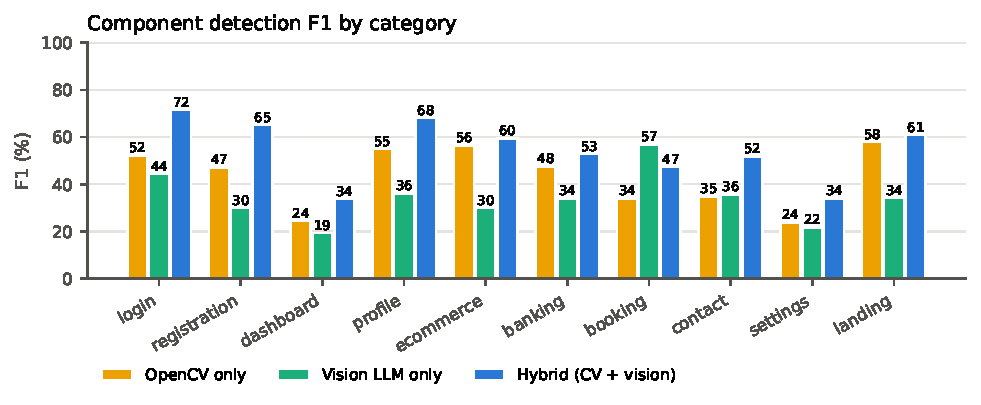
\includegraphics[width=\columnwidth]{figures/eval/detection_f1_by_category.pdf}
\caption{Detection F1 per screen category for each analysis mode and for the rendered DOM of both systems.}
\label{fig:detcat}
\end{figure}

\subsection{Voice Command Accuracy}
Whisper transcribes the synthesised commands with a corpus word error rate of \WhisperWerPipeline{}\%. From the Whisper transcript, \VoiceCommandAccuracyPipeline{}\% of commands are interpreted fully correctly (operation, target and parameters); from the reference text the figure is 93.8\% (Table~\ref{tab:voice}). Per category, add, remove, style, interaction and navigation are interpreted almost perfectly; resize is the weakest (60\% from the transcript) because quantities such as ``a bit bigger'' are ambiguous. Speech recognition errors cost about 2.6 percentage points relative to clean text (91.2\% vs.\ 93.8\%); we did not analyse which tokens were misrecognised.

\begin{table}[t]
\centering
\scriptsize
\caption{Voice command interpretation accuracy (\%)}
\label{tab:voice}
\setlength{\tabcolsep}{3.5pt}
\begin{adjustbox}{max width=\columnwidth}
\begin{tabular}{lrrrrr}
\toprule
\textbf{Input} & \textbf{Commands} & \textbf{Op type} & \textbf{Target} & \textbf{Parameters} & \textbf{All correct} \\
\midrule
Ground-truth text & 80 & 97.5 & 97.5 & 98.6 & 93.8 \\
Whisper transcript & 80 & 96.2 & 97.5 & 95.7 & 91.2 \\
\bottomrule
\end{tabular}
\end{adjustbox}
\end{table}


\subsection{Generated UI Quality}
Table~\ref{tab:quality} reports visual and functional quality. The generated UI renders in 100\% of cases for both systems. Layout IoU against the sketch is 0.399 for the proposed pipeline and 0.283 for the baseline; the compiler's oracle ceiling is 0.593. Edge SSIM is nearly identical (0.52 vs.\ 0.51), so the two systems look equally similar to the sketch at the pixel-structure level; the gain is in component placement. Functional correctness is \FunctionalCorrectnessPipeline{}\% vs.\ \FunctionalCorrectnessBaseline{}\%, and the difference is almost entirely in navigation (92\% vs.\ 72\% of 25 specified interactions). Validation and message behaviours are equal. Requirement satisfaction is at parity (\RequirementSatisfactionPipeline{}\% vs.\ \RequirementSatisfactionBaseline{}\%); the baseline is better at honouring specific input types (97.1\% vs.\ 91.2\%).

\begin{table*}[t]
\centering
\scriptsize
\caption{Generated UI quality: visual similarity, functional correctness, requirement satisfaction}
\label{tab:quality}
\setlength{\tabcolsep}{3.5pt}
\begin{adjustbox}{max width=\textwidth}
\begin{tabular}{lrrrrrr}
\toprule
\textbf{System} & \textbf{Sketches} & \textbf{Renders \%} & \textbf{Layout IoU} & \textbf{Edge SSIM} & \textbf{Functional \% (n)} & \textbf{Requirements \% (n)} \\
\midrule
Proposed (NeuroGenUI) & 40 & 100.0 & 0.399 & 0.522 & 94.8 (58) & 87.5 (407) \\
Proposed, before repair & 40 & 100.0 & 0.399 & 0.522 & 94.8 (58) & 87.5 (407) \\
Baseline (sketch$\rightarrow$AI$\rightarrow$UI) & 40 & 100.0 & 0.283 & 0.509 & 86.2 (58) & 86.0 (407) \\
Oracle (GT IR) & 40 & 100.0 & 0.593 & 0.551 & 6.9 (58) & 85.3 (407) \\
\bottomrule
\end{tabular}
\end{adjustbox}
\end{table*}


\begin{figure}[t]
\centering
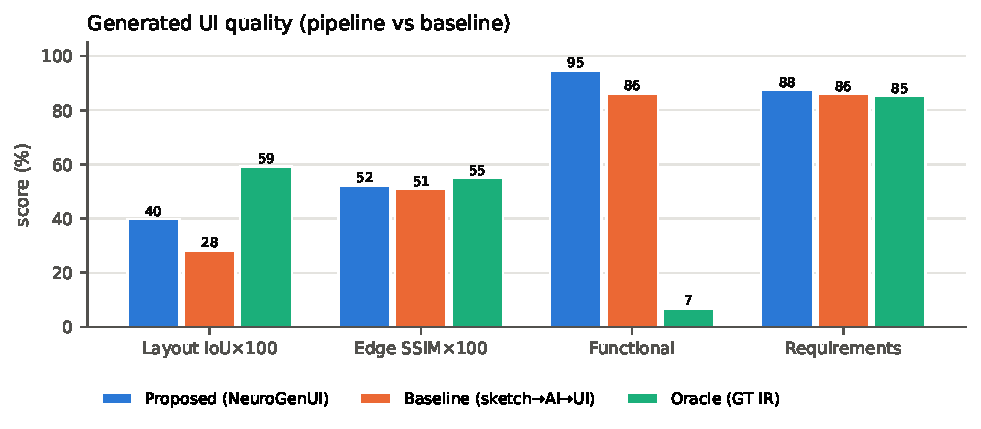
\includegraphics[width=\columnwidth]{figures/eval/generation_quality.pdf}
\caption{Generated UI quality: pipeline, baseline and the ground-truth oracle.}
\label{fig:quality}
\end{figure}

\subsection{Voice-Guided Refinement}
Table~\ref{tab:refine} shows refinement success and preservation per command category. The proposed pipeline applies \RefinementSuccessRatePipeline{}\% of commands successfully against \RefinementSuccessRateBaseline{}\% for the baseline (93.8\% when the command goes through Whisper), a difference of four commands out of 80 that we do not claim as significant. The categories differ: the pipeline is better on add, style, navigation and resize; the baseline is better on modify and move (100\% on both). The clearer difference is preservation. Because refinements are operations on the existing IR, \PreservationRatePipeline{}\% of unaffected components are unchanged in type, text, colour, size and font, against \PreservationRateBaseline{}\% when the baseline regenerates the program. Latency differs by an order of magnitude: \ModificationTimeMsPipeline{}\,s on average for the pipeline (one short interpretation call plus deterministic edit and compile) against \ModificationTimeMsBaseline{}\,s for a full regeneration.

\begin{table*}[t]
\centering
\scriptsize
\caption{Refinement success and preservation (\%) per command category}
\label{tab:refine}
\setlength{\tabcolsep}{3.5pt}
\begin{adjustbox}{max width=\textwidth}
\begin{tabular}{lrrrrrr}
\toprule
\textbf{Category} & \textbf{Success: Proposed (NeuroGenUI)} & \textbf{Success: Proposed, Whisper transcript} & \textbf{Success: Baseline (sketch$\rightarrow$AI$\rightarrow$UI)} & \textbf{Preserved: Proposed (NeuroGenUI)} & \textbf{Preserved: Proposed, Whisper transcript} & \textbf{Preserved: Baseline (sketch$\rightarrow$AI$\rightarrow$UI)} \\
\midrule
add & 100.0 & 100.0 & 80.0 & 100.0 & 100.0 & 96.3 \\
remove & 100.0 & 100.0 & 100.0 & 99.4 & 99.4 & 98.9 \\
modify & 90.0 & 90.0 & 100.0 & 100.0 & 100.0 & 100.0 \\
move & 80.0 & 80.0 & 100.0 & 100.0 & 100.0 & 94.1 \\
resize & 90.0 & 80.0 & 70.0 & 99.1 & 98.2 & 99.2 \\
style & 100.0 & 100.0 & 90.0 & 100.0 & 100.0 & 97.1 \\
interaction & 100.0 & 100.0 & 100.0 & 100.0 & 100.0 & 100.0 \\
navigation & 100.0 & 100.0 & 80.0 & 100.0 & 100.0 & 100.0 \\
all & 95.0 & 93.8 & 90.0 & 99.8 & 99.7 & 98.2 \\
\bottomrule
\end{tabular}
\end{adjustbox}
\end{table*}


\subsection{Validation and Repair}
After the development fixes described in Section~\ref{sec:dev}, \ValidationPassRateBeforeRepairPipeline{}\% of generated UIs pass validation before repair, so on this test set the repair loop is not triggered during normal generation and we cannot measure a pass-rate improvement. We therefore evaluate validation and repair directly by \emph{fault injection} (Table~\ref{tab:faults}): across 438 injected faults on pipeline and oracle UIs, the validator detects \FaultDetectionRatePipeline{}\% and the repair loop restores \FaultRepairRatePipeline{}\%. Detection is strong for hidden, zero-size, reordered and broken-event faults. Repair is reliable for broken event handlers (100\%) and reordering (97.5\%) but weak for hidden nodes (42.5\% on pipeline UIs) and deleted nodes (55\%), so the loop is not a general recovery mechanism. Deleting a node is also the fault the validator detects least often on pipeline UIs (75\%); we did not investigate why.

\begin{table}[t]
\centering
\scriptsize
\caption{Fault injection: validator detection and repair recovery (\%)}
\label{tab:faults}
\setlength{\tabcolsep}{3.5pt}
\begin{adjustbox}{max width=\columnwidth}
\begin{tabular}{lrrrrr}
\toprule
\textbf{IR source} & \textbf{Fault} & \textbf{Cases} & \textbf{Detected \%} & \textbf{Localised \%} & \textbf{Repaired \%} \\
\midrule
oracle & delete\_node & 40 & 95.0 & 95.0 & 77.5 \\
oracle & hide\_node & 40 & 100.0 & 100.0 & 52.5 \\
oracle & zero\_size & 40 & 100.0 & 100.0 & 65.0 \\
oracle & swap\_order & 40 & 100.0 & 62.5 & 97.5 \\
oracle & code\_error & 40 & 100.0 & 100.0 & None \\
oracle & all & 200 & 99.0 & 91.5 & 73.1 \\
pipeline & delete\_node & 40 & 75.0 & 60.0 & 55.0 \\
pipeline & hide\_node & 40 & 100.0 & 100.0 & 42.5 \\
pipeline & zero\_size & 40 & 95.0 & 95.0 & 75.0 \\
pipeline & swap\_order & 40 & 100.0 & 50.0 & 97.5 \\
pipeline & break\_event & 38 & 100.0 & 100.0 & 100.0 \\
pipeline & code\_error & 40 & 100.0 & 100.0 & None \\
pipeline & all & 238 & 95.0 & 84.0 & 73.7 \\
\bottomrule
\end{tabular}
\end{adjustbox}
\end{table}


\begin{figure}[t]
\centering
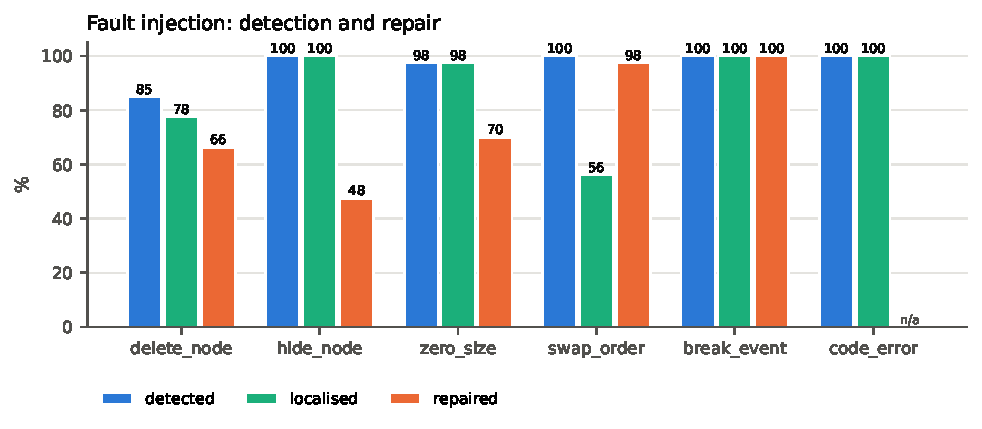
\includegraphics[width=\columnwidth]{figures/eval/fault_injection.pdf}
\caption{Fault injection: share of injected faults detected, localised and repaired, by fault type.}
\label{fig:faults}
\end{figure}

\subsection{Generation Time}
The proposed pipeline produces a usable UI in \GenerationTimeMsPipeline{}\,s on average (median 10.7\,s) against \GenerationTimeMsBaseline{}\,s for the baseline, including validation and repair (16.4\,s). Table~\ref{tab:latency} breaks this down: sketch analysis (10.4\,s mean, dominated by the vision call) and interpretation (5.1\,s) account for almost all of it, while fusion, code generation and validation together take about 0.5\,s. Latencies include network time to the model API and vary with load.

\begin{table}[t]
\centering
\scriptsize
\caption{Latency per stage (ms)}
\label{tab:latency}
\setlength{\tabcolsep}{3.5pt}
\begin{adjustbox}{max width=\columnwidth}
\begin{tabular}{lrrrrr}
\toprule
\textbf{System} & \textbf{Stage} & \textbf{n} & \textbf{Mean} & \textbf{Median} & \textbf{p95} \\
\midrule
pipeline & analyze\_sketch & 40 & 10350 & 5890 & 10705 \\
pipeline & interpret & 40 & 5114 & 4987 & 7215 \\
pipeline & fuse & 40 & 3 & 3 & 6 \\
pipeline & codegen & 40 & 1 & 1 & 2 \\
pipeline & total\_generate & 40 & 15469 & 10654 & 18343 \\
pipeline & validate & 40 & 517 & 443 & 703 \\
pipeline & repair & 40 & 460 & 442 & 667 \\
pipeline & total\_with\_validation & 40 & 16446 & 11563 & 19432 \\
baseline & total\_generate & 40 & 23968 & 16976 & 65240 \\
analyze\_cv & analyze\_cv & 40 & 66 & 55 & 103 \\
analyze\_vision & analyze\_vision & 40 & 6445 & 6237 & 8711 \\
analyze\_hybrid & analyze\_hybrid & 40 & 10350 & 5890 & 10705 \\
pipeline & modify\_total & 80 & 2103 & 2063 & 2708 \\
pipeline\_voice & modify\_total & 80 & 2104 & 2106 & 2676 \\
baseline & modify\_total & 80 & 15360 & 13883 & 23314 \\
\bottomrule
\end{tabular}
\end{adjustbox}
\end{table}


\subsection{Code Quality}
Both systems produce code that parses in all cases (Table~\ref{tab:code}). Generated code from the proposed compiler is organised in reusable components: each definition is used 1.85 times on average against 1.01 for the baseline, which inlines most elements. The baseline's longest function averages 206 lines against 106 for the proposed code, and the exported project is split into multiple files. ESLint reports almost no messages for either system (0.05 vs.\ 0.03 per UI). The compiler's longest function grew from 57 to 106 lines between the development run and the final run, after geometry-aware layout was added.

\begin{table*}[t]
\centering
\scriptsize
\caption{Static code quality of the generated React (mean per UI)}
\label{tab:code}
\setlength{\tabcolsep}{3.5pt}
\begin{adjustbox}{max width=\textwidth}
\begin{tabular}{lrrrrrrrr}
\toprule
\textbf{Code} & \textbf{UIs} & \textbf{Parses \%} & \textbf{LOC} & \textbf{Components} & \textbf{Reuse ratio} & \textbf{Max function lines} & \textbf{ESLint msgs} & \textbf{Files} \\
\midrule
Proposed (NeuroGenUI) [project] & 40 & 100.0 & 410.8 & 13.9 & 1.85 & 105.6 & 0.0 & 17.9 \\
Proposed (NeuroGenUI) [preview] & 40 & 100.0 & 379.0 & 13.9 & 1.85 & 105.6 & 0.1 & 1.0 \\
Baseline (sketch$\rightarrow$AI$\rightarrow$UI) [preview] & 40 & 100.0 & 246.3 & 1.4 & 1.01 & 206.1 & 0.0 & 1.0 \\
Oracle (GT IR) [preview] & 40 & 100.0 & 307.6 & 11.6 & 1.60 & 76.1 & 1.0 & 1.0 \\
\bottomrule
\end{tabular}
\end{adjustbox}
\end{table*}


\section{Discussion}
\subsection{Development Iteration}
\label{sec:dev}
The first full evaluation (Run~1) was run on the first complete version of the system and exposed real defects, which we then fixed and re-evaluated on the same test set (Table~\ref{tab:dev}). In Run~1 only 42.5\% of generated UIs passed validation; none of the 43 repair actions applied during generation fixed anything; navigation commands succeeded for 3 of 10 cases; the compiler stacked all components in one column, so rendered-DOM detection F1 was \DevComponentDetectionFODomPipeline{}\% and layout IoU \DevVisualSimilarityLayoutIouPipeline{}\%, below the baseline on both. The causes were respectively empty or placeholder-less components that rendered invisibly, a repair step that reset styles instead of fixing the cause, a navigation target the refinement step failed to read from the operation, and a compiler that ignored the sketch geometry already stored in the IR. We fixed these with general changes (placeholder content in fusion, targeted repair actions, geometry-aware layout, global fusion matching) rather than changes specific to individual sketches.

Because the fixes were guided by the same test set, the final numbers are \emph{development-set} results: the improvement from Run~1 to the final run demonstrates that the evaluation exposes real defects, but it overstates what we should expect on unseen sketches. A held-out set drawn by different people would be required for an unbiased estimate.

\begin{table}[t]
\centering
\scriptsize
\caption{Development iteration: the first full evaluation exposed pipeline defects that were fixed (Sec.~\ref{sec:dev}); same test set}
\label{tab:dev}
\setlength{\tabcolsep}{3pt}
\begin{adjustbox}{max width=\columnwidth}
\begin{tabular}{lrrr}
\toprule
\textbf{Metric} & \textbf{Run 1} & \textbf{Final} & \textbf{Baseline} \\
\midrule
Component detection F1 (analysis vs.\ baseline DOM) & 42.9 & 53.1 & 25.6 \\
Component detection F1 (both on rendered DOM) & 16.5 & 42.9 & 25.6 \\
Visual similarity: layout IoU $\times$100 & 20.5 & 39.9 & 28.3 \\
Functional correctness & 91.4 & 94.8 & 86.2 \\
Refinement success rate & 81.2 & 95.0 & 90.0 \\
Validation pass rate before repair & 42.5 & 100.0 & -- \\
Validation pass rate after repair & 42.5 & 100.0 & -- \\
Injected faults repaired & 60.7 & 73.5 & -- \\
\bottomrule
\end{tabular}
\end{adjustbox}
\end{table}


\subsection{What the Results Support}
The measurements support three claims. (i)~Combining OpenCV geometry with a vision model detects more components than either alone, and the structured pipeline recovers more of the sketched components in rendered UIs than a single-call baseline (F1 \ComponentDetectionFODomPipeline{}\% vs.\ \ComponentDetectionFODomBaseline{}\%). (ii)~Representing the UI explicitly makes refinement cheap and local: operations on the IR take about \ModificationTimeMsPipeline{}\,s, preserve \PreservationRatePipeline{}\% of unaffected components and are as successful as full regeneration (\RefinementSuccessRatePipeline{}\% vs.\ \RefinementSuccessRateBaseline{}\%, not separable on 80 commands). (iii)~Validation in a real browser detects most injected faults (\FaultDetectionRatePipeline{}\%) and repair restores about three quarters of them. The measurements do \emph{not} show that the pipeline produces visually closer UIs in an absolute sense (layout IoU 0.40 against a compiler ceiling of 0.59), that it satisfies requirements better (parity), or that the repair loop improves generation pass rates (it was not needed on this set).

\subsection{Limitations}
\label{sec:limits}
\begin{itemize}
\item \textbf{Synthetic data.} Sketches are procedurally rendered in a hand-drawn style and commands are synthesised speech; results on real drawings, varied handwriting and real voices (accents, noise) are expected to be lower.
\item \textbf{Single run, small test set.} We report one run on \CountSketches{} sketches and \CountCommands{} commands without confidence intervals; model-API variation and heuristic DOM extraction add noise (re-measuring identical cached baseline code moved two baseline numbers by 0.1--0.2 points).
\item \textbf{Tuned on the test set.} See Section~\ref{sec:dev}.
\item \textbf{Heuristic measurement.} Components are recovered from the rendered DOM by tags, roles and visual cues. The procedure is identical for both systems, but it can miss or mis-type components for either.
\item \textbf{One model family.} Perception and interpretation use one hosted model and one speech model; the baseline and the pipeline share it, but conclusions may differ for other models.
\item \textbf{Deletion and hidden-node faults} are the weakest cases for detection and repair, and sketch detection still misses about 42\% of components (recall 58.2\% at the analysis stage).
\item \textbf{Scope.} The system targets a controlled vocabulary of common components, single-user use, front-end-only behaviour (no backend generation) and English commands.
\end{itemize}

\subsection{Future Work}
Collecting sketches from real users and recorded speech would give an unbiased evaluation. Learned detectors fine-tuned on UI datasets could replace the geometric proposals, and the intent model could be extended with clarification questions for ambiguous commands such as relative resizing. The compiler could target additional frameworks, and the validator could add accessibility and responsiveness checks. A user study of the studio, comparing time to a satisfactory UI against direct prompting, would measure what the latency and preservation advantages mean in practice.

\section{Conclusion}
We presented NeuroGenUI, a multimodal framework that turns a hand-drawn sketch and spoken instructions into an editable React interface through an explicit UI Intent Representation, refines it by voice with local operations, and validates and repairs it in a real browser. On \CountSketches{} synthetic sketches and \CountCommands{} spoken commands, the staged pipeline detected more of the sketched components in rendered UIs than a direct sketch$\rightarrow$AI$\rightarrow$UI baseline, satisfied more interactions, and applied refinements about seven times faster with higher preservation, while matching the baseline on requirement satisfaction and refinement success. An initial evaluation also exposed defects that were fixed and re-measured, which we report as a development iteration. The main open problems are detection recall on real hand drawings and robust recovery from deleted or hidden components. The code, dataset and evaluation scripts are provided so that every number in this paper can be reproduced.


\bibliographystyle{IEEEtran}
\bibliography{refs}

\end{document}
